\documentclass{sig-alt-release2}
\usepackage{url}
\usepackage{color}
\usepackage{graphics,graphicx}

\usepackage{aeguill}

\usepackage{epsfig}
\usepackage{epstopdf}

\usepackage{colortbl}
\usepackage{multirow}
\usepackage{booktabs}
\usepackage{ifthen}  

\begin{document}
\newcommand{\todo}[1]{\textcolor{red}{#1}}
\def\newblock{\hskip .11em plus .33em minus .07em}

\conferenceinfo{DIM3} {2012, Glasgow, UK} 
\CopyrightYear{2012}
\clubpenalty=10000
\widowpenalty = 10000

\title{{Where in the BOB?}}

\numberofauthors{4}
\author{
Andrei Palade, 0907350, 0907350p@student.gla.ac.uk\\
Andrei Mustata, 0907390, 0907390m@student.gla.ac.uk\\
Cristian Urlea, 1102465, 1102465u@student.gla.ac.uk \\
Wei Zhang, 1104733, 1104733z@student.gla.ac.uk\\
\\
          \affaddr{\textbf{Group F, DIM3}}\\
    %  \affaddr{Dim3}\\
%      \affaddr{Student no.s}\\
 %            \email{\{ 0907350, 0907390, 1102465, 1104733\}
  %           @students.glasgow.ac.uk }
}

\maketitle

\begin{abstract}

\textbf{Where in the BOB?} is a simple web application that enables users to
find the location of a room in the Boyd Orr Building. 
   
This application aims to provide a simple interface where the user inserts the
name of a room in a text field and as a result he gets a floor map in \texttt{SVG}
format with the room highlighted. It provides a list of room names in case of
an ambiguous identifier and the ability to give comments on a particular room. 

\end{abstract}

\section{Aim of Application}

The application name is ``Where in the BOB'' and its purpose is to provide
students, lecturers and visitors of University of Glasgow with an identifying
system of rooms located in Boyd Orr Building. The application intends to
offer a \todo{customize} interface to this facility where a particular user has the
options to view from a floor plan perspective the location of a given room,
to view details about the room searched and provide comments and ratings of
the room in cause. \todo{Moreover, the application will offer details if the room
or the floor is accessible or not.}

The \todo{assumption}, in this case, is to build such a system based on the provided
floor plans of the building. Furthermore, the search facilities are restricted
to a given number of most well know room names amongst students (e.g. Level 3
Computer Science lab) as well as their official names(e.g. Room 720). In this
case, if the room is identified, the result of the search will contain a floor
plan with the location of the searched room highlighted, details about the
room (e.g. number of seats, other details of access, comments on the room),
otherwise it will return a message to confirm that the search process has
failed to identify that particular room (i.e. The rooms was not identified).

\subsection{Goals}
Another goal is to provide the user with a list of room names in case that
there are multiple rooms across campus especially in the Boyd Orr Building.
A particular goal which will provide the user with a consistent and optimized
results is to:
\begin{itemize}
	\item  search again in case of not found 
	\item  leave feedback
	\item  comment on room 
\end{itemize}


\subsection{Assumptions}

We made a number of assumptions based on the purpose of this web application. 
It is assumed that users have a minimum knowledge of English and have the basic 
knowledge of how to use a web browser as well as having Internet connection on 
the used devices.

The visual interaction with the application makes it necessary for the user to 
be able to see and to use one hand in order to interact with the device as they 
do with other applications. This include holding a mouse in order to move a 
pointer around the screen or using fingers to point to different parts of the 
screen on touchscreen handheld devices.

Another assumption we made is that users will be students or visitors with 
minimal knowledge about the campus and they use their handheld device for 
coordination around campus.



\subsection{Constraints}

\subsubsection{Development constraints}

The major constraint we are concerned about is the time necessary to develop 
the application. We will use the available time during the labs to implement 
the required functionality of our system and we will also make use of Django 
web framework for fast development. Due to budgetary constraints we are forced 
to use open source software which cause another issue in terms of technical 
knowledge regarding the tools used.

\subsubsection{Application constraints}
\begin{itemize}
	\item \textbf{End-user environment}: The end-user system can be deployed
	on a wide range of devices (e.g. desktop or mobile systems). These devices
	come with a restricted screen size.
	\item \textbf{Hardware}: 
	\item \textbf{Network}:
	\item \textbf{Interface/Protocol}:
\end{itemize}




\subsection{Functionality}
The required and desired functionality of our application is as follows:
\begin{itemize}
	\item The required functionality:
	\begin{itemize}
		\item Accept textual search terms and return results for a searched
		room identifier 
		
		\item Provide a graphical view of the room that is being searched
		within Boyd Orr Building
		
		\item Return an SVG format of the floor plan where the searched
		room is located with the room highlighted
		
		\item Return a list of matching results for ambiguous defined
		identifiers
		
		\item Allow users to leave comments for a the searched room		
	\end{itemize}

	\item The desired functionality:
	\begin{itemize}
		\item Allow users to see the floor map directory
		\item Allow users to search give feedback on the application
		\item Allow users to return and search for a different room
		\item Allow users to check the accessibility of the room
	\end{itemize}
\end{itemize}

\section{Client Interface}

We have tried to design a user interface that is very intuitive, making it
easy for the users to find what they're looking for.

\subsection*{Wireframes}
All the pages will have the basic layout of the \textbf{Home} page
(Figure \ref{img:wireframes-home}), which consists of:
\begin{itemize}
	\item{
		\textbf{Header}
		\begin{enumerate}
			\item{
				\textbf{Name} of the website
			}
			\item{
				\textbf{Tagline}/short description of how the app works, so
				the users won't have to go through the tedious process of
				reading through an \textbf{About} page
			}
			\item{
				\textbf{Search box} - this is where the users input their
				query
			}
		\end{enumerate}
	}

	\item{
		\textbf{Content} - the rest of the page will be displayed in this area
	}
	
	\item{\textbf{Footer} - contains the links for the \textbf{navigation menu}
	}
\end{itemize}


The pages \textbf{Results} and \textbf{Directory} share the same design (Figure 
\ref{img:wireframes-results}): a list of all the levels, and for each one of 
them, a list of rooms. If a query returns more than one result, this page is 
shown with the list of matching rooms. In the case of the Directory page, all 
the levels are listed. Their elements are:
\begin{enumerate}
	\item{\textbf{Query} - the searched term}
	\item{\textbf{Result set} - the results of the query grouped by the level
	they're on}
\end{enumerate}


The pages for \textbf{floors} are very similar to the ones for particular
\textbf{rooms} (Fig. \ref{img:wireframes-room}), the only difference being that
instead of the breadcrumbs that appear on the room page, the floor page only 
displays the floor number. The structure of these pages:
\begin{enumerate}
	\item{\textbf{Breadcrumbs} Level number + room number, in the case of 
	the room page.}
	\item{\textbf{Floor map} - for the room page, the particular room is
	highlighted.}
	\item{\textbf{Comment form} - small \texttt{textarea} and a 
	\texttt{Submit} button.}
	\item{\textbf{Comments} - previous comments (text + date posted)}
\end{enumerate}

\subsection*{User classes}
This section presents a use case analysis of the website. The use cases 
presented here model the interaction between users and the website. These use 
cases will be used to guide usability, to provide a task-oriented 
documentation system.

There will be 2 user classes:
\begin{itemize}
	\item \textbf{Visitor} - end users of the system;
	\item \textbf{Administrator} - techy, but not much
\end{itemize}

\subsubsection*{Visitor}
Visitors are the \textbf{end-users} of the application. They could be either
new students who are not used to the University's campus yet, or anyone else
who can't find their way through the complex system of rooms and hallways that
is the Boyd Orr Building.

\emph{``I'm a level 2 CS student and I can't find my way to the lab. All 
I know is I should be in the \guillemotleft Level 2 lab in the Boyd Orr
\guillemotright. Now, I've managed to find the \textbf{floor}, but I'm not sure
which room I need to go to. Oh,look! There's a room directory up on the wall, 
but it's not very helpful. I sure wish there was an app for this, lol!''}

His goal is to find information regarding a particular room (e.g.: what floor 
it is on, where exactly it is on that floor, etc). He might know the room 
number or some other unofficial name for that room.

They can ask the application about different rooms in the BOB. If that room 
name exists, the app shows an image with the appropriate floor plan and the 
searched room is highlighted.

\subsubsection*{Administrator}
Someone needs to manage all that data, so there will be an administrator. He is
responsible for maintaining the database (room labels, floor plans).

\subsubsection*{User matrix}
\begin{tabular}{| p{4cm} | p{1cm} | p{1cm}|} \hline
\textbf{Functionality} & \textbf{Visitor} & \textbf{Admin} \\ \hline
Browse directory & X & X \\ \hline
Search for a room & X & X \\ \hline
Post comment & X & X \\ \hline
Send feedback & X & X \\ \hline
Edit/Delete Comment & & X \\ \hline
Add/edit floor &  & X \\ \hline
Add/edit room & & X \\ \hline
Add/edit floor plan & & X \\ \hline

\end{tabular}	


\section{Application Architecture}

\subsection*{N-tier architecture}
The N-tier architecture (Figure \ref{img:arch-ntier}) blahblahblah.

The \textbf{presentation tier} is the topmost layer of the application,
represented by the user interface. It translates user actions into commands
for the application and it presents the information retrieved by the app in a
way that the user can understand.

\todo{\textbf{Logic/application tier}}

\todo{\textbf{Data tier}}

\subsection*{ERD}

\todo{The ERD} (Figure \ref{img:arch-erd}).

\todo{Tables}

\begin{tabular}{| p{2cm} | p{2cm} | p{3cm}|}
\hline
Data name & Data type & Rationale \\
\hline
id & Integer & Unique ID to identify each floor \\
\hline
description & String & Room description used to supply extra details to optimize the search\\
\hline
date\_created & Date & The floor plan was added\\
\hline
date\_updated & Date & The floor plan was last updated\\
\hline
level & Integer & Optimize the search and reduce the fetch time\\
\hline
rating & Integer & Optimize the search by using popularity\\
\hline
GUID & Integer & Unique ID for the comment\\
\hline
\end{tabular}	


\section{Message Passing}

\begin{figure}
        % \begin{center}
                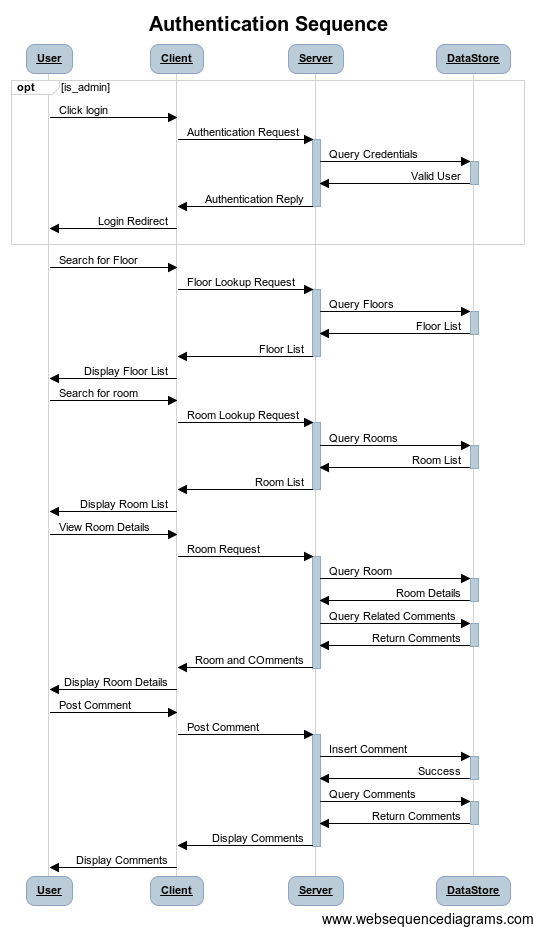
\includegraphics[scale=0.35]{img/dia.png}
                \caption{Sequence Diagram.}
                \label{img:diagram-sequence}
        % \end{center}
\end{figure}

\todo{Sequence diagram}

\todo{Messages, lol}


\section{Summary and Future Work}
\begin{itemize}
\item	Summary of application and its current state.
\item	Include a list or table of all the technologies, standards, and protocols that will be required.
\item	What are the limitations?
\item Plans for future development
\end{itemize}

\section{Acknowledgements}
Our thanks to the lecturers and demonstrators for their comments and suggestions. And our thanks to the peer reviewers for their feedback.
Be sincere and be specific about how others have helped your group.

\bibliographystyle{abbrv}
\bibliography{sig-proc}

\section{Appendix}
\begin{figure}
\begin{minipage}[b]{0.5\linewidth}\centering
        % \begin{center}
                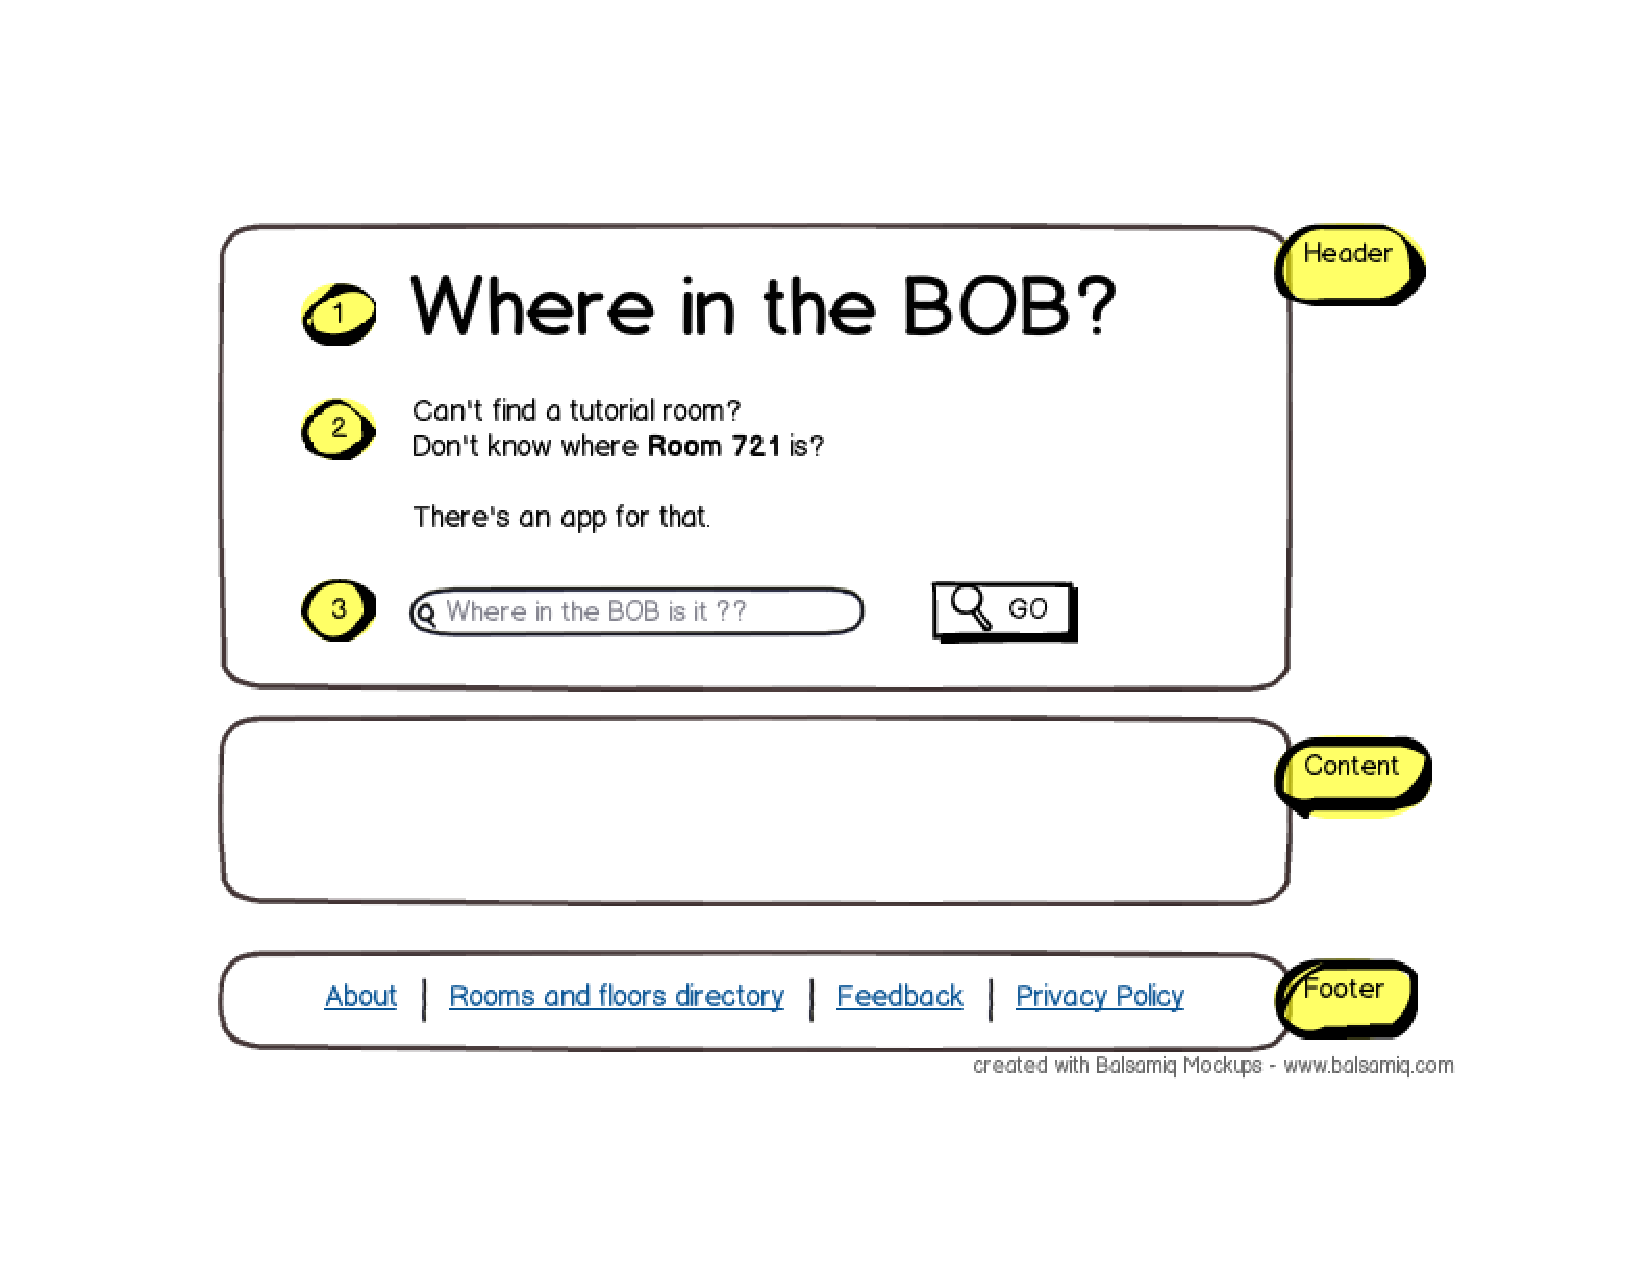
\includegraphics[scale=0.35]{img/wireframes/home.pdf}
                \caption{Wireframe for the Home page.}
                \label{img:wireframes-home}
        % \end{center}
\end{minipage}
%\end{figure}
%\begin{figure}
\hspace{4cm}
\begin{minipage}[b]{0.5\linewidth}\centering
        % \begin{center}
                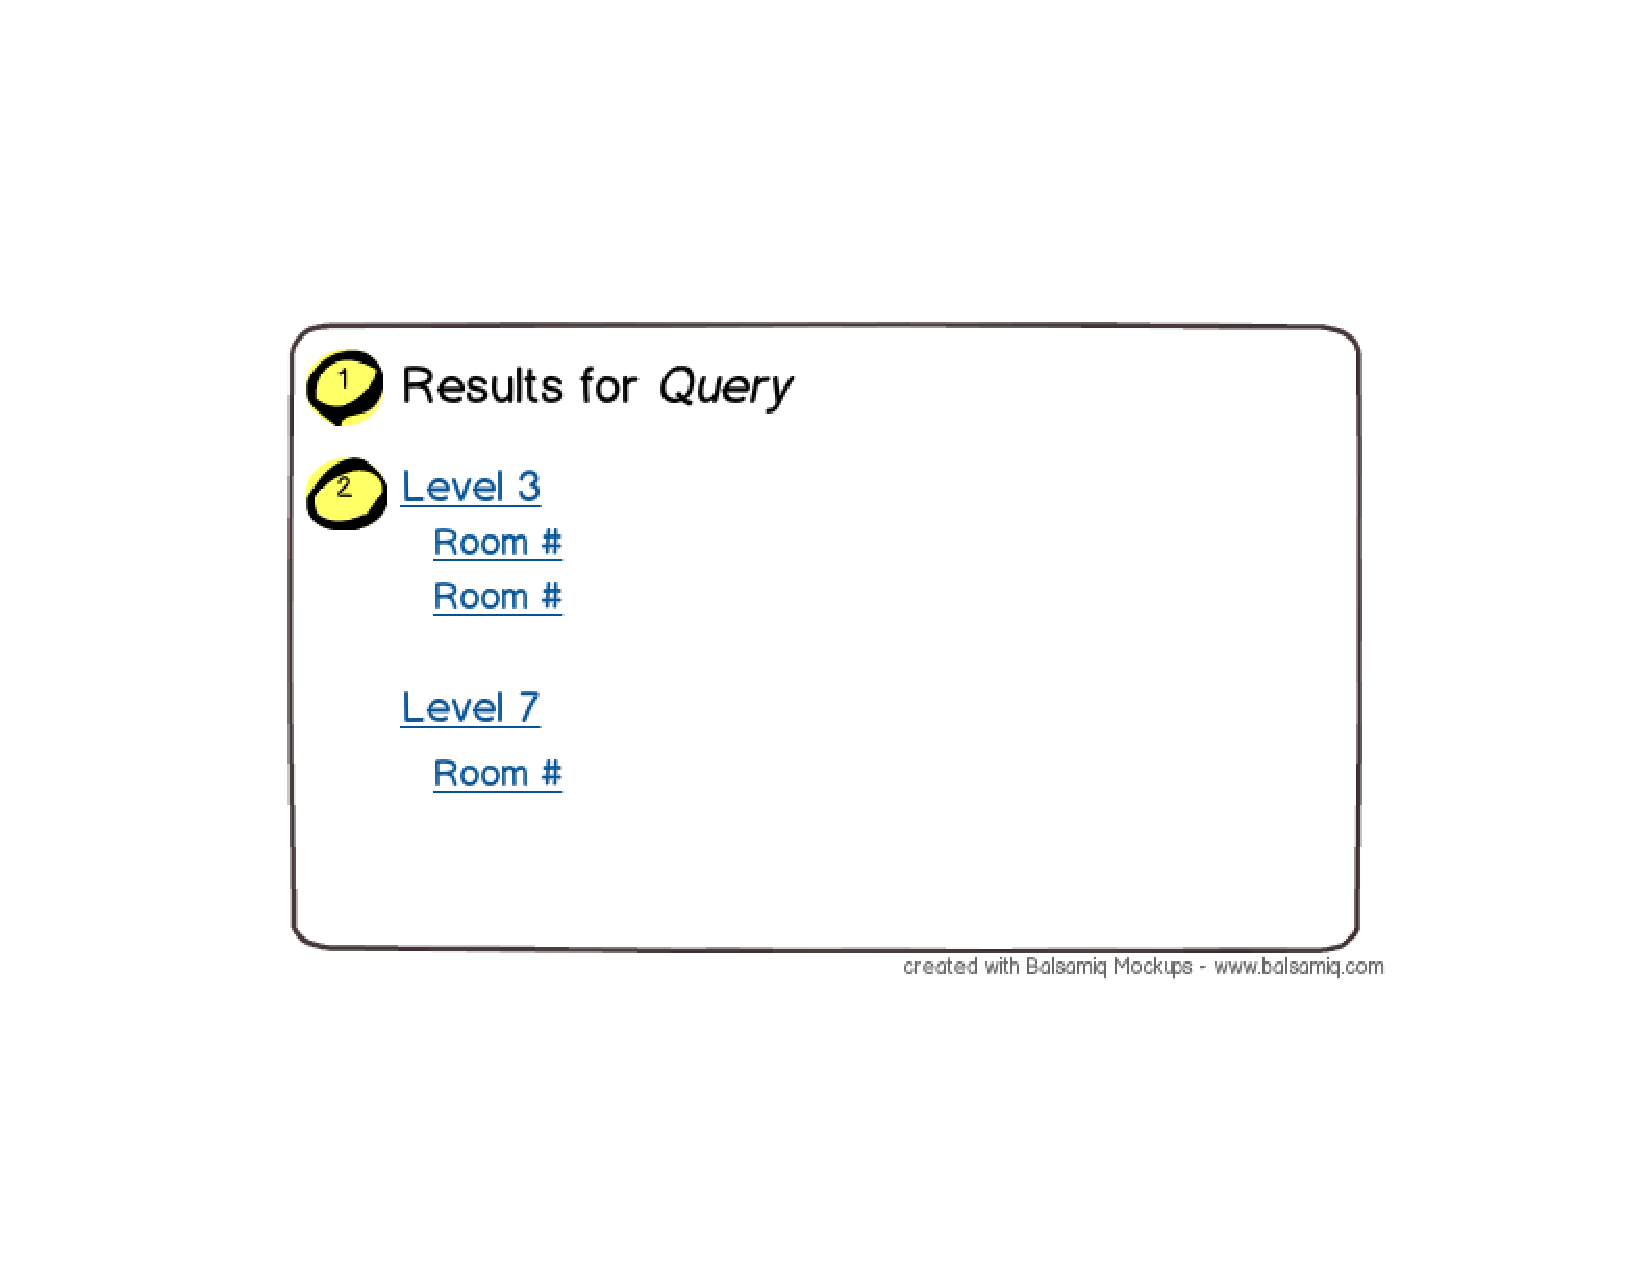
\includegraphics[scale=0.35]{img/wireframes/results.pdf}
                \caption{Wireframe for the Results/Directory page.}
                \label{img:wireframes-results}
        % \end{center}
\end{minipage}
\end{figure}


%\begin{figure}
%\begin{minipage}[b]{0.5\linewidth}\centering
        % \begin{center}
%                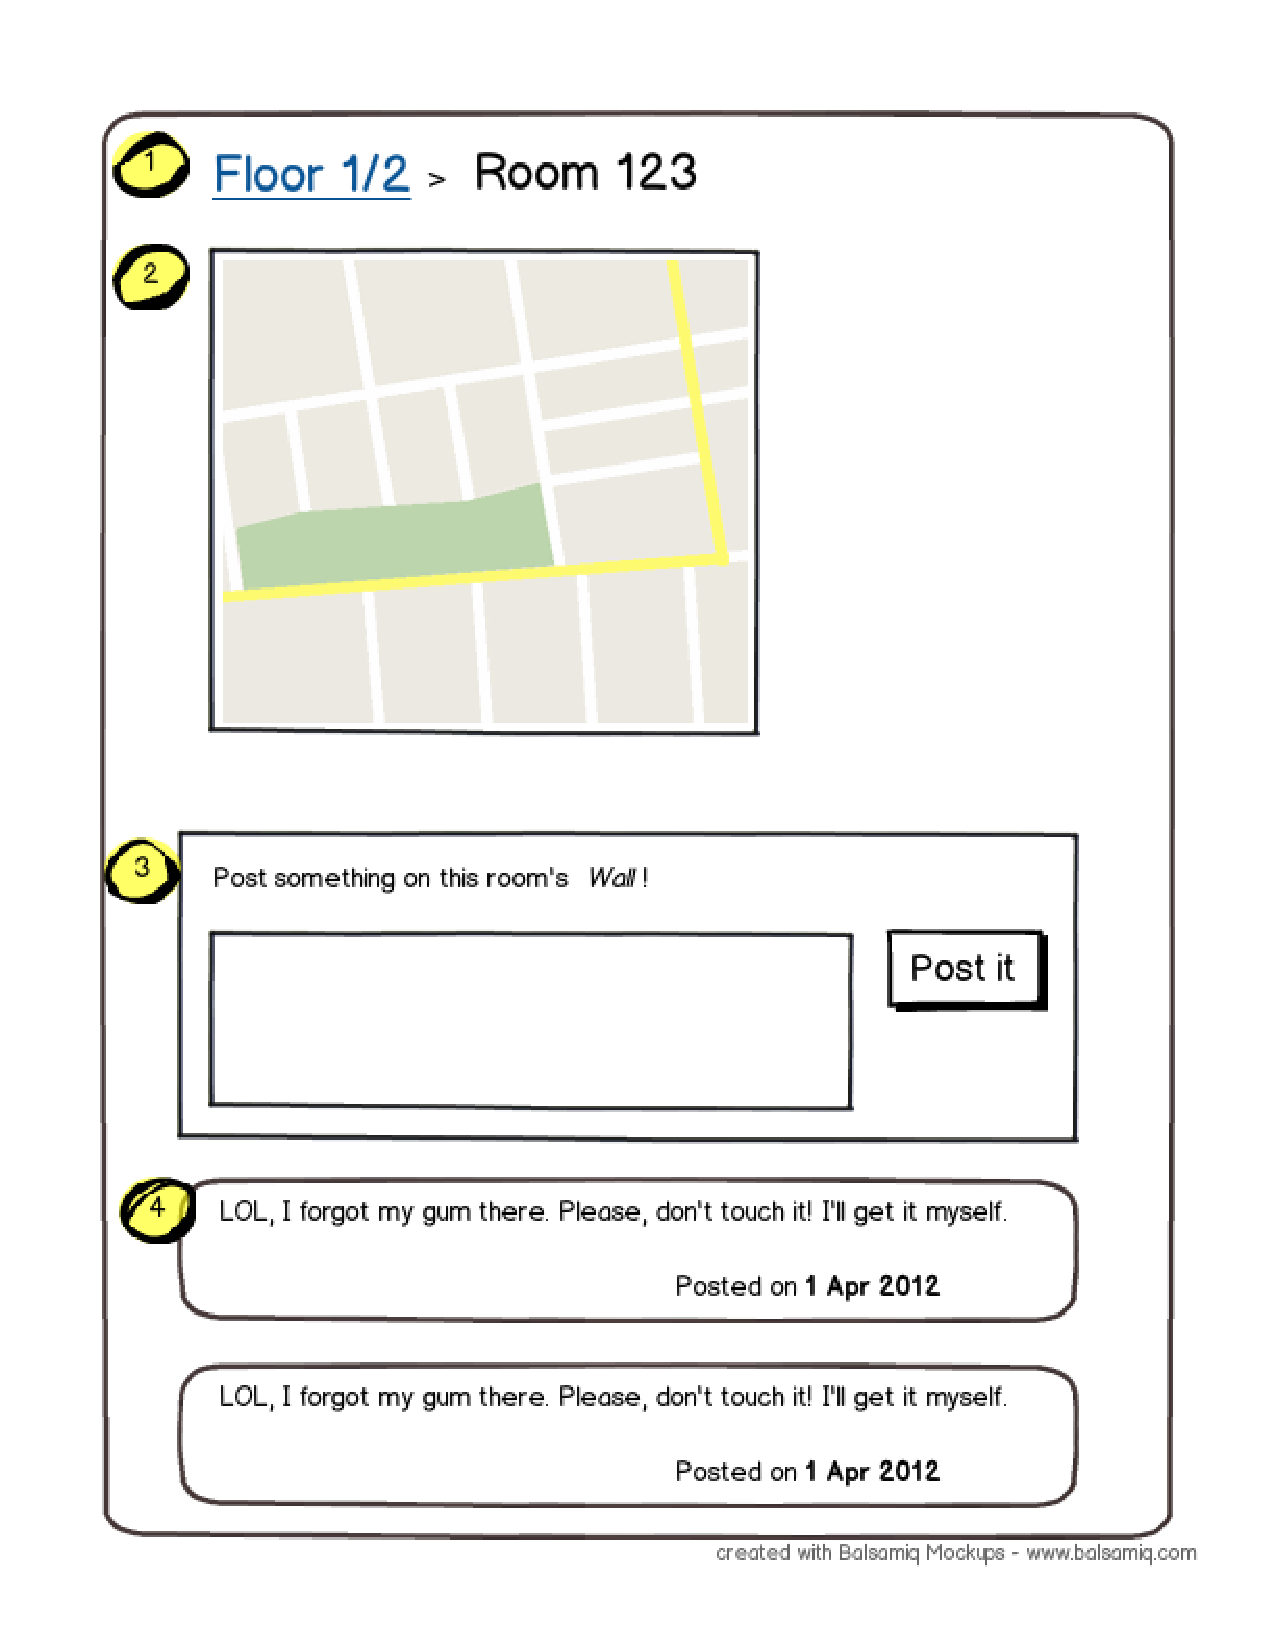
\includegraphics[scale=0.35]{img/wireframes/room.pdf}
%                \caption{Wireframe for the Room/Floor page.}
%                \label{img:wireframes-room}
        % \end{center}
%\end{minipage}
%\end{figure}
%\begin{figure}
%\hspace{4cm}

%\begin{minipage}[b]{0.5\linewidth}\centering

        % \begin{center}
%                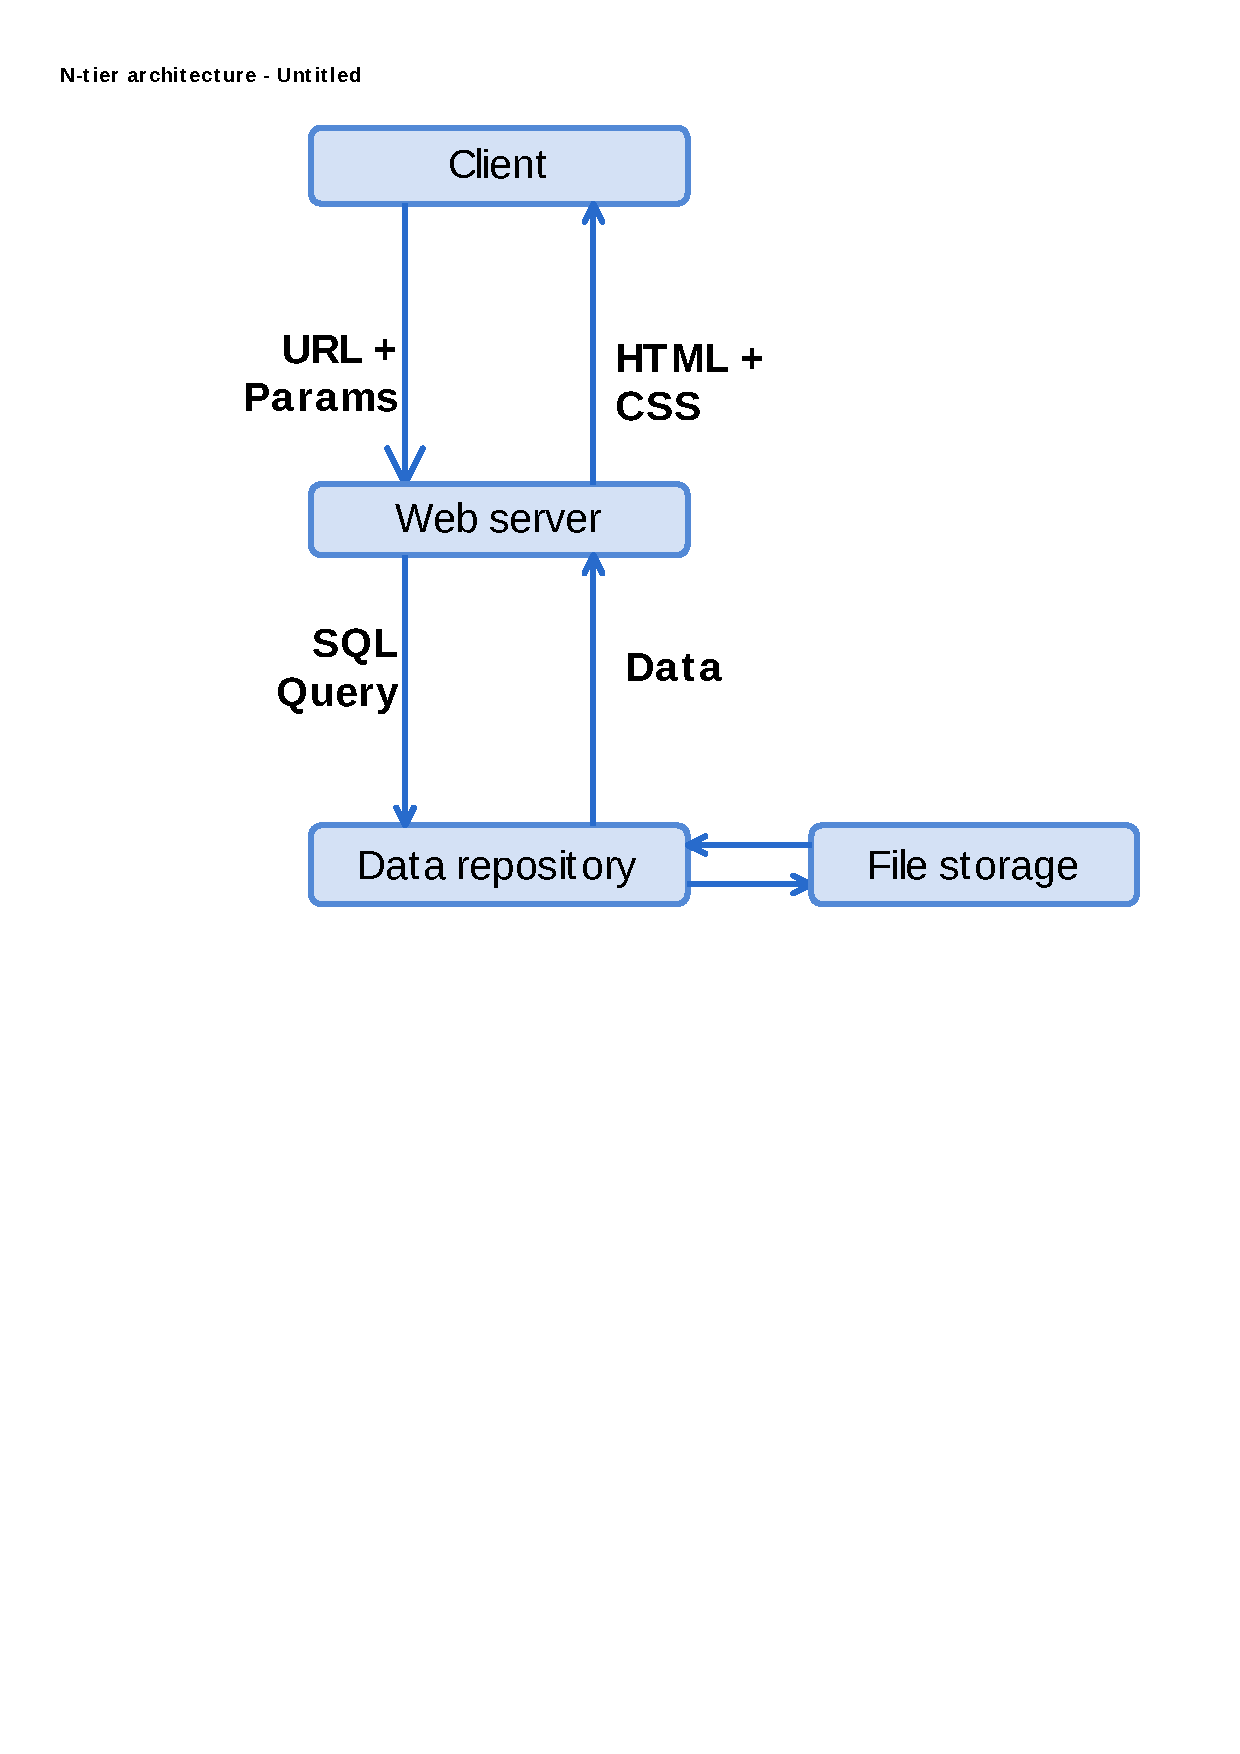
\includegraphics[scale=0.35]{img/ntier.pdf}
%                \caption{N-tier architecture.}
%                \label{img:arch-ntier}
        % \end{center}
%\end{minipage}
%\end{figure}
%\begin{figure}
        % \begin{center}
                % 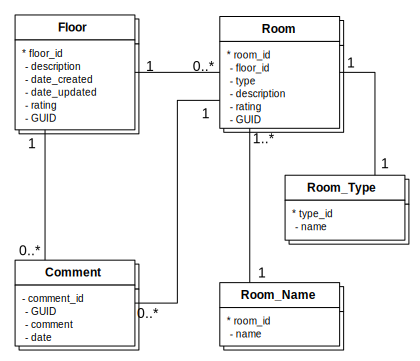
\includegraphics[scale=0.35]{img/erd.pdf}
%                \caption{ERD.}
%                \label{img:arch-ntier}
        % \end{center}
%\end{figure}
%\begin{figure}
        % \begin{center}
%                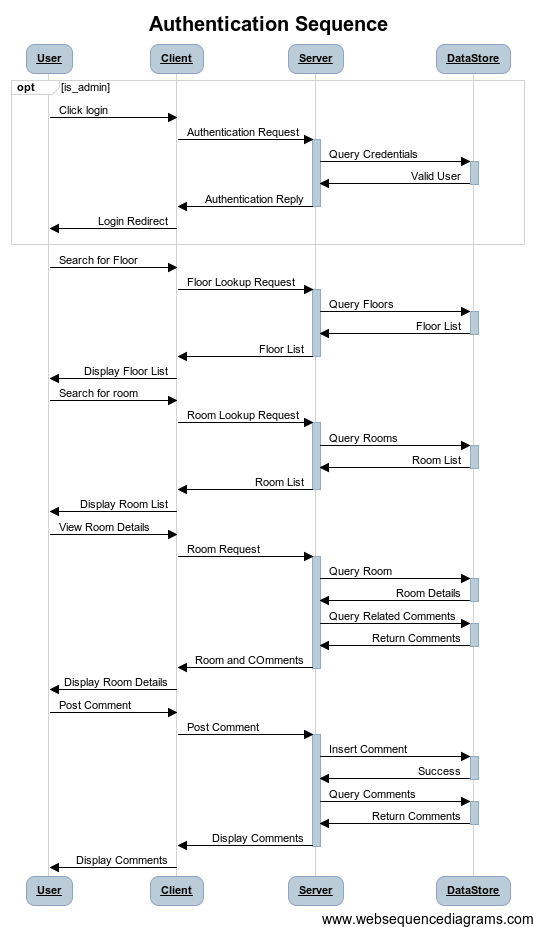
\includegraphics[scale=0.35]{img/dia.png}
%                \caption{Sequence Diagram.}
%                \label{img:diagram-sequence}
        % \end{center}
%\end{figure}


\end{document}
